% !TEX root = ../thesis.tex
\chapter{Progenitor search in SN 1006}
\label{chap:sn1006}


\section{Introduction}

The search for a donor star in \sn{1572}\ has not turned up an obvious candidate. However, we have detected two objects (\starb\ and \starg) exhibiting some unusual properties, which while interesting, ultimately seem inconsistent with the expectations of any viable donor star scenario. Since donor star scenarios are theoretical in their nature and any actual donor star is likely to not exhibit all features predicted by the model. We have reached an impasse with \sn{1572}{} and more detailed observations will likely not provide a definitive answer if either of these two stars were involved in the progenitor system. An obvious way forward is to scrutinize stars in other \snia\ remnants and see if any of those have similar properties to \starb\ or \starg. The remnant of \sn{1006}{} is the ideal object for this kind of follow-up search. 

The lack of a central neutron star, observation of several 0.1\,\msun\ of iron inside the remnant \cite{1997ApJ...481..838H} and the the high peak luminosity and basic light curve shape \citep[visible for several years][]{1965AJ.....70..748G} all indicate that \sn{1006}{} was a \snia. In addition, the remnant has a secure distance, measured by \citet{2003ApJ...585..324W}, who combined the proper motion and the radial velocity of the expanding shell to measure the distance to 2.2\,\kpc, making \sn{1006}{} the closest of the ancient \snia\ remnants (consistent \sn{1006}{} being the brightest).   The geometric center of the remnant has been determined from both \xray\ and radio observations \citep{2003ApJ...585..324W}. The interior of the remnant has been probed with UV background sources \citep{2005ApJ...624..189W}. This revealed the aforementioned iron core as well as a silicon rich shell. The remnant has been searched for possible \snia\ donor stars previously, and an unusual O-star has been previously identified as a possible donor star to \sn{1006}{}.

This unusual O-Star was identified near the centre of \sn{1006}{} by \citet{1980ApJ...241.1039S} and is now called Schweizer-Middleditch Star (\smstar). After successful identifications of neutron stars in both the Vela Remnant and the Crab Remnant this was thought to be the third identification of a stellar remnant in ancient supernovae. Subsequent UV spectroscopic follow-up of the \smstar\ by \citet{1983ApJ...269L...5W} , showed strong \ion{Fe}{2}  with a profile broadened by a few thousand \kms. In addition, \citet{1983ApJ...269L...5W} identified redshifted \ion{Si}{2}, \ion{Si}{3} and \ion{Si}{4} lines. Their conclusion was that these absorption lines stem from the remnant and place the \smstar\ behind the remnant, making it unrelated to \sn{1006}{}. Although unrelated, the \smstar\ is an ideal object to probe the remnant and measure upper limits for interstellar extinction \citep[E(B-V) = 0.1][]{1993ApJ...416..247W,2003ApJ...585..324W}.


SN 1006 has several properties which make it an ideal place to undertake a progenitor search.  Although the remnant is the oldest among the known \snia\ remnants, its age is still young enough that  the remnant's center is well determined, and the motion of any donor star small enough that only a small area of stars need to be searched. Furthermore, this elapse of 1005 years is a short length of time relative to the timescales of stellar evolution for donor stars \cite[see][]{2000ApJS..128..615M}. We still expect a potential donor star to be close to the same state as directly after the supernova explosion. In addition, \sn{1006}{} has a low interstellar extinction, which makes the determination of stellar parameters much less challenging. These serendipitous conditions for the \sn{1006}{} remnant led us to launch a photometric and spectroscopic campaign to search for the donor star. Our photometric observations were taken at Siding Spring Observatory with the 2.3m Telescope imager. The spectroscopic observations were undertaken with the high resolution multi-object spectrograph FLAMES attached to the \gls{vlt}.


In Section \ref{sec:obs_red} we outline the observations as well as data reduction of the photometric and spectroscopic data. Section \ref{sec:sn1006_analysis} is split into four subsections, namely radial velocity, stellar rotation and stellar parameters. We conclude this chapter in Section \ref{sec:conclusion} and discuss the possible implications of our initial find as well as outlining some future work.


\section{Observations and Data Reduction}
\label{sec:obs_red}
Our photometry was obtained from images taken with the imager at the 2.3m Telescope at the Siding Spring Observatory. All data was taken on the night of the 11th of May 2004. We exposed for 1860\,s in U-Band, 1490\,s in B-Band, 788\,s in V-Band and 1860\,s in I-Band. For calibration purposes we took images of the PG1633 and PG1047 standard star regions in the same filters. The seeing ranged between 1\arcsec and 2\arcsec. 
The data was reduced in the standard way using PyRAF \footnote{PyRAF is a product of the Space Telescope Science Institute, which is operated by AURA for NASA.}.

For the spectroscopy survey we chose the \gls{vlt} instrument FLAMES, which provides high resolution (R=25,000) and a large field of view (25\arcmin) for 130 targets although with a small spectral coverage of 200\,\AA. We chose the wavelength region from 5139\,\AA\ to 5356\,\AA\ which contains the gravity sensitive \gls{mgb} Triplet as well as many iron lines to accurately measure metallicity. As the centre of our spectroscopic survey we chose the mean of the \xray\ and radio center \citep[$\alpha = \rasc{15}{02}{22}{1};\delta = \decl{-42}{05}{49}$][]{2003ApJ...585..324W}. We chose a search radius of 120\arcsec which corresponds to 1250\,\kms at 2.2\,\kpc. This generous choice, which is more than four times our maximum expected escape velocity (see Figure \ref{fig:han2008_vrad}), was made to accommodate any errors in the choice of the center. Although the models predict the surviving companion to be several hundred \lsun\ \citep{2000ApJS..128..615M}, we chose a limiting magnitude of $V=17.5$ ($0.5\,\lsun(V)$ at 2.2\,\kpc\ including extinction of E(B-V)=0.1) to have a comfortable margin of error. An exposure time of 3.8 hours was chosen to obtain spectra with high enough quality to measure rotation and basic stellar parameters (\snratio\ $>20$) For completeness and to not waste fibres we chose additional stars down to a magnitude limit of $V=19$, which are only used in radial velocity measurements. These constraints yielded 26 stars with $V<17.5$ and 53 stars in the bin between $17.5<V<19$ (for a total of 79 stars) for our survey (see Figure \ref{fig:overview_sn1006}). With fibre buttons not being able to be placed less than 11\arcsec\ apart, we had to split our candidates over three different setups. The first two setups were observed five times with 2775 s each. We deliberately chose bright stars for the last setup so that it only had to be observed three times with 2775 s each. As only the central 120\arcsec were crowded we placed spare fibres on three bright stars (R$\approx 10$; 2MASS J15032744-4204463, 2MASS J15031746-4204165, 2MASS J15033195-4202356) located close to the edge of the 25\arcmin\ field of view for calibration purposes. Additional spare fibres were placed on sky positions. These were configured to be placed far from \twomass\ sources and were subsequently manually inspected using \gls{dss} images to be in star free regions. 
\begin{figure}[htbp] %  figure placement: here, top, bottom, or page
   \centering
   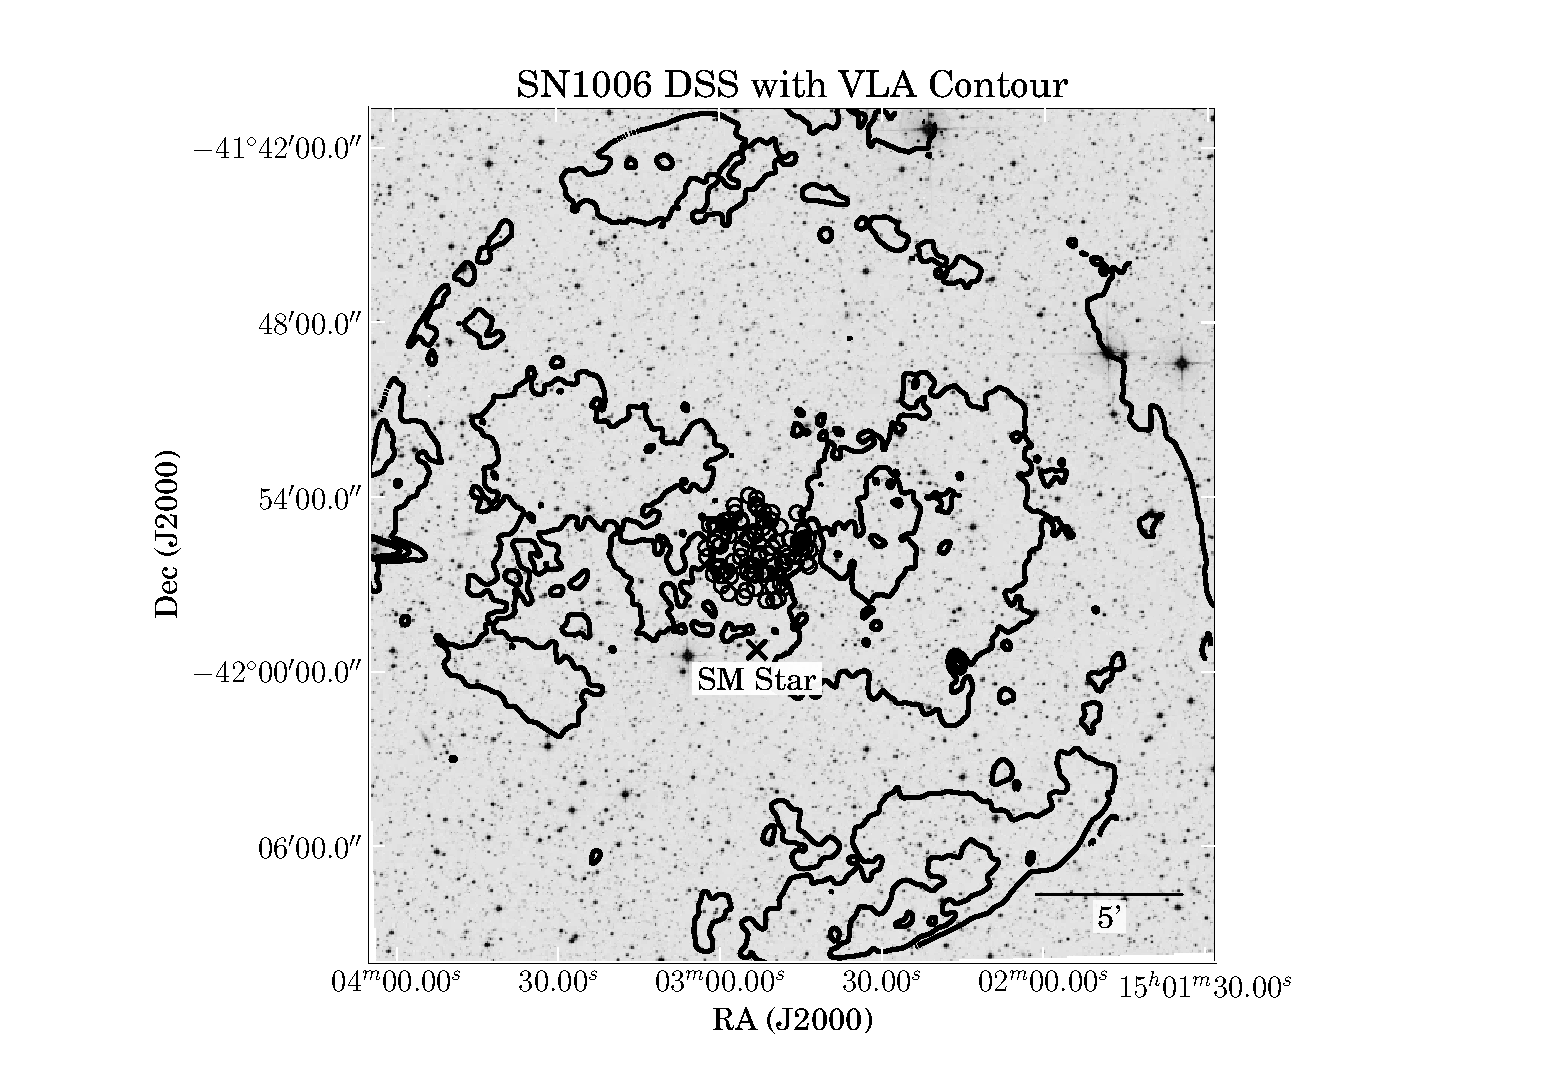
\includegraphics[width=0.8\textwidth]{chapter_sn1006/plots/sn1006_overlay_withsm.pdf} 
   \caption[Overview of candidates and remnantin SN 1006]{Optical DSS image with radio contour overlay (VLA). The black circles in the center show the 79 program stars. Additionally we have marked the `spurious` donor the \smstar.}
   \label{fig:overview_sn1006}
\end{figure}
In addition to our night time calibration, which included simultaneous arc exposures with four fibres for each observation block, we received standard daytime calibrations. In total, 13 observation blocks with an exposure time of 2775 s each were obtained. Table \ref{tab:observations} provides the Observing ID, modified julian date, mean seeing, mean airmass, setup name and heliocentric correction for all observations (all data is available under ESO Program ID: 083.D-0805(A)). Due to broken fibres not all stars where observed for the expected length of time. Broken fibres caused \candstar{31} not to be observed at all in this sample (see Figure \ref{fig:zoomed_overview_sn1006}). On the other hand \candstar{31} with $V=17.87$ is also not considered a candidate.
\begin{deluxetable}{cccccc}
\tablecaption{Observations}
\tablehead{\colhead{ObsID} & \colhead{MJD} & \colhead{FWHM} & \colhead{Airmass} & \colhead{SetupName} & \colhead{$\Delta v_{\rm helio}$}\\ 
\colhead{-} & \colhead{d} & \colhead{\arcsec} & \colhead{-} & \colhead{-} & \colhead{\kms}}


\startdata
360737 & 54965.1 & 1.2 & 1.2 & SN1006 1 & 1.5\\
360739 & 54965.1 & 1.2 & 1.1 & SN1006 1 & 1.5\\
360740 & 54965.1 & 1.0 & 1.1 & SN1006 1 & 1.4\\
360741 & 54985.0 & 0.7 & 1.4 & SN1006 1 & -7.4\\
360742 & 54964.2 & 1.5 & 1.1 & SN1006 1 & 1.7\\
360743 & 54985.0 & 0.8 & 1.2 & SN1006 2 & -7.5\\
360745 & 54985.0 & 0.9 & 1.1 & SN1006 2 & -7.6\\
360746 & 54985.1 & 1.0 & 1.1 & SN1006 2 & -7.7\\
360747 & 54985.1 & 1.0 & 1.1 & SN1006 2 & -7.7\\
360748 & 54985.2 & 0.9 & 1.1 & SN1006 2 & -7.8\\
360749 & 54963.1 & 1.2 & 1.2 & SN1006 3 & 2.4\\
360751 & 54963.1 & 1.1 & 1.1 & SN1006 3 & 2.3\\
360752 & 54963.2 & 1.1 & 1.1 & SN1006 3 & 2.3\\
\enddata
\label{tab:observations}
\end{deluxetable}


\begin{figure}[htbp] %  figure placement: here, top, bottom, or page
   \centering
   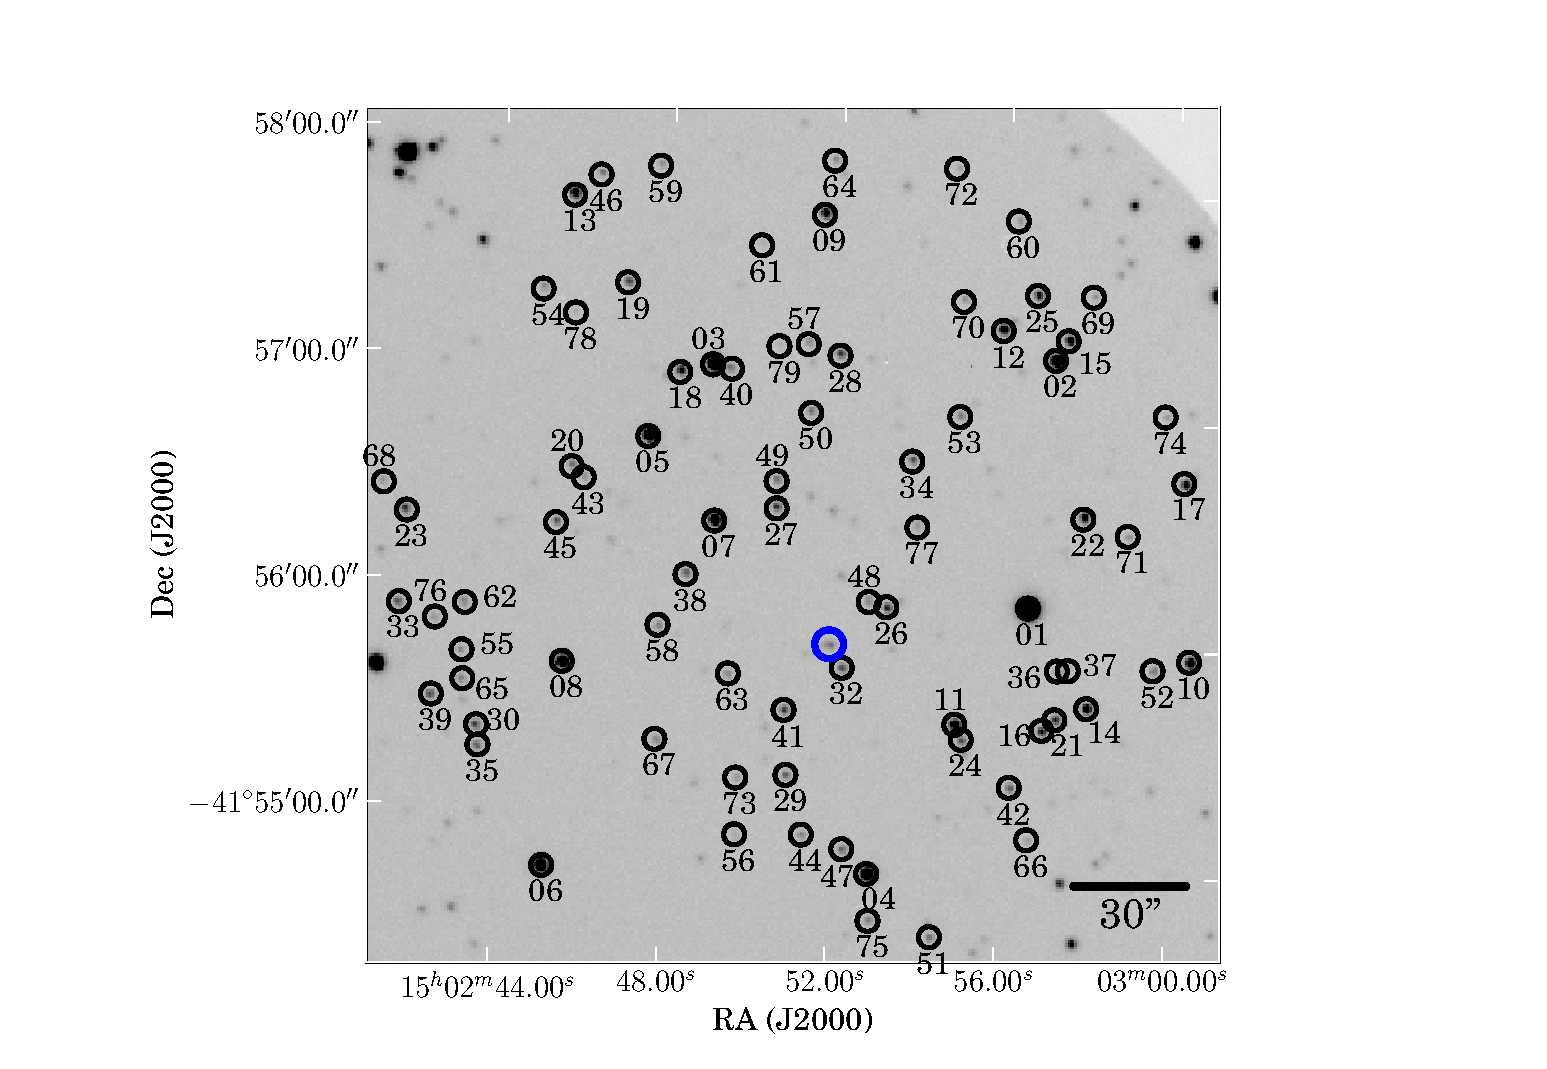
\includegraphics[width=0.8\textwidth]{chapter_sn1006/plots/overview_labeled_sn1006.pdf} 
   \caption[Close-up of the candidates in SN 1006] {V-Band image taken by the 2.3m Telescope. We have marked \candstar{31}, which was not observed due to broken fibres, with a blue circle. With the a brightness of V=17.87 \candstar{31} is much fainter than \lsun(V) at the distance of 2.2\,\kpc and would not be considered a donor star candidate.}
   \label{fig:overview_sn1006}
\end{figure}


We first applied a cosmic ray removal tool on the raw 2D frames \citep{2001PASP..113.1420V}. The data was then reduced with the ESO-CPL pipeline (version 5.2.0), using the GIRAFFE instrument recipes (version 2.8.9). The only change that was made to the default parameters was the usage of the Horne extraction algorithm instead of the "Optimal"-extraction algorithm. This yielded 366 individual spectra of the candidate stars and an additional 39 spectra of the Calibration stars. 

For our photometric data reduction we fitted an astrometric solution using astrometry from the \twomass\ point source catalogue \citep{2006AJ....131.1163S} to our frames. 
We used SExtractor \citep{1996A&AS..117..393B} to measure the magnitudes of the objects in the frames and then calibrated our photometry to a standard Bessel Filter system using the Stetson magnitudes \footnote{This research used the facilities of the Canadian Astronomy Data Centre operated by the National Research Council of Canada with the support of the Canadian Space Agency}  of our standard fields PG1633 and PG1047 .  

The measured magnitudes were supplemented with near infrared magnitudes from the \twomass\ point source catalogue (see Table \ref{tab:sn1006_twomass} and \ref{tab:sn1006_photometry} ). Subsequently we checked the photometric measurements, by plotting the obtained $B-V$ colours against the $V-K$ colours (see Figure \ref{fig:colour_check}).
\begin{figure}[htbp] %  figure placement: here, top, bottom, or page
   \centering
   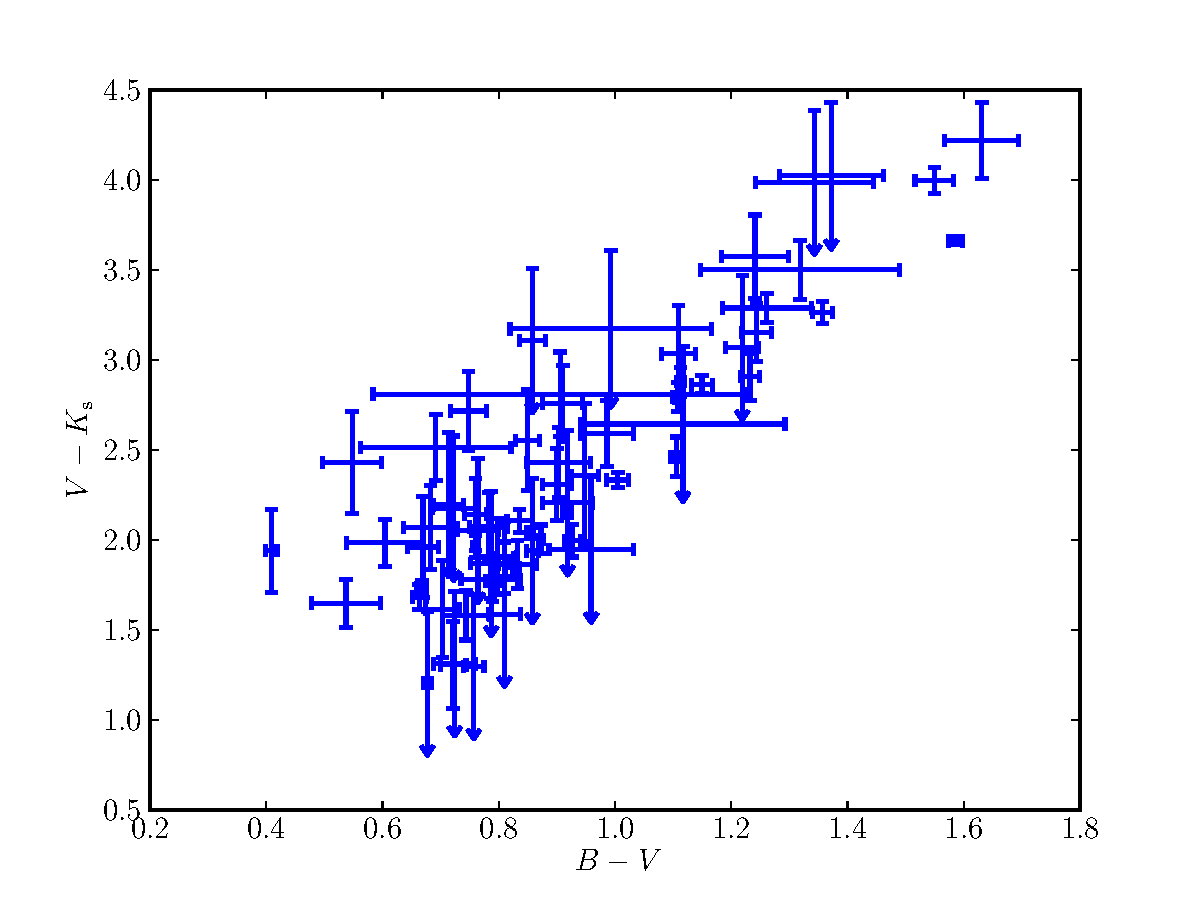
\includegraphics[width=0.7\textwidth]{chapter_sn1006/plots/color_bv_vk.pdf} 
   \caption[Colour-colour plot of all candidates in SN 1006 to check photometry]{Colour-colour plot of all candidates in SN 1006 to check photometry. Considering the error bars and upper limits for some stars all of the objects lie pretty well on the stellar locus}
   \label{fig:colour_check}
\end{figure}

We have also computed temperatures from photometric colours by using the polynomials given in \citet{2010A&A...512A..54C}. We assumed an \gls{feh} of 0 for all stars, but the choice of \gls{feh} only has a minor influence on the temperature calculation (e.g. change of 300K between \gls{feh}=0 and \gls{feh}=-1) for the temperature. In addition, the temperature polynomial coefficients incorporating the metallicity are particularly small for the $V-K$ colour. All temperatures are listed in the optical photometry Table \ref{tab:sn1006_photometry} and infrared photometry Table \ref{tab:sn1006_twomass}.


\section{Analysis}
\label{sec:sn1006_analysis}
\subsection{Radial Velocity}

\begin{figure}[tb] %  figure placement: here, top, bottom, or page
   \centering
   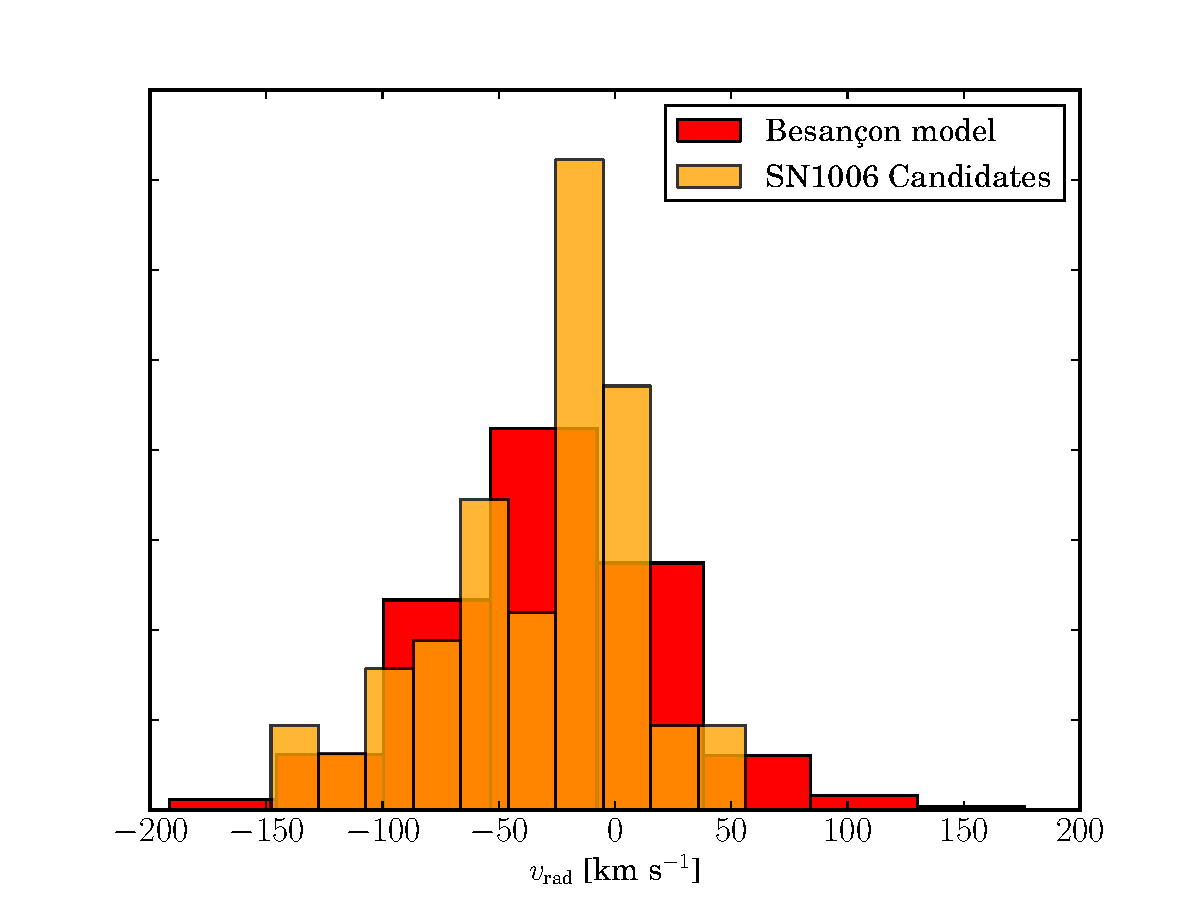
\includegraphics[width=0.7\textwidth]{chapter_sn1006/plots/sn1006_vrad_besancon.pdf} 
   \caption[Radial velocity of all candidates in SN 1006 compared with Besan\c{c}on Model]{Comparison of all candidate stars with the distribution of stars taken from the the Besan\c{c}on kinematic model. The model input parameters were a search area of 1 square degree around the center of \sn{1006}{} and a magnitude limit of $10<\textrm{V}<17.5$}
   \label{fig:sn1006_vrad_comp}
\end{figure}


To obtain radial velocities we employ a two step process. We used a solar spectrum from \citet{1984sfat.book.....K} with the standard cross-correlation technique described in \citet{1979AJ.....84.1511T} and implemented in the IRAF task \textit{fxcor}. The cross-correlation was performed on every single spectra. The results were then heliocentrically corrected, then averaged for each star with a sigma clipping algorithm (see Table \ref{tab:sn1006_kinem}). We note that especially for faint objects we observe a second cross-correlation peak at 0\,\kms and believe that this is reflected light from the moon. We believe that this has a negligible effect on our radial velocity measurement.
In Figure \ref{fig:sn1006_vrad_comp} we have compared our radial velocity measurements with the Besan\c{c}on kinematic model of the Milky way \citep{2003A&A...409..523R}. Our selection criteria for creating the  Besan\c{c}on kinematic model was all stars within 1 square degree of \sn{1006}{} and a magnitude cut of $10<\textrm{V}<17.5$. We compared the resulting 10000 stars to our 78 stars in the sample. 




\subsection{Rotational Velocity}
\label{sec:sn1006_rotvel}
Due to the direction looked through the galaxy, there is a large velocity spread in the direction of \sn{1006}{} (see Figure \ref{fig:sn1006_vrad_comp}). This makes it hard to isolate a donor star based just on kinematic features. A distinguishing feature for a donor star might be rotation (discussed in Chapter \ref{chap:sn1572_starg}). The rotational velocities in Chapters \ref{chap:sn1572_starg} \& \ref{chap:sn1572_hires} were all measured manually. We selected weak iron lines and stacked them to obtain a line profile, which was compared to synthetically rotationally broadened lines. This was a feasible way for six spectra, it is however not feasible for more than 200 spectra. 

Initially we had tried to fit the rotational velocity as an additional parameter in the determination of stellar parameters. For the fainter spectra the optimization algorithm suggested very high rotations. A simple manual inspection revealed that this was not the case.  
%Initially we tried a simple fourier transform of the spectra without using a window function. This caused a very noisy fourier spectrum, which was hard to analyse. 
%\cite{citeulike:8297810} describes a very robust method to obtain periodic information of spectra.  He suggests dividing the spectra into overlapping subsegments. These are then multiplied with a window function (in our case ``Hann''-window) and transformed into the fourier domain. All fourier segments are then averaged, which provides a very clean fourier spectrum. Figure \ref{fig:sn1006_psd} shows the periodogram of synthetic spectra with different rotation and different S/N-ratios. For synthetic data this methods worked even for a S/N of roughly 5. Measuring rotation in our real data remained too difficult in the low S/N regime. 

%picture: This reduces removes the low frequencies and reduces frequency resolution. In our case, however, we are interested in high frequency caused by the line profiles. 
We realized that in Fourier space it becomes much easier to determine repetitive  structures like line profiles. For a description of this method, however we need to review part of the spectral synthesis. The intrinsic spectrum ($f_\textrm{spectrum}$) is created at the photosphere of the star (but already broadened by many factors like thermal broadening and natural broadening). Additionally, the rotation of that star convolves the spectrum with a rotational broadening kernel ($g_\textrm{rotation}$). The light travels to earth and then is convolved again with the instrumental profile ($h_\textrm{instrument}$) before being recorded on the detector.  Let's assume we can create a synthetic spectra matching the intrinsic stellar one which has not been convolved by either rotation or the instrument ($f_\textrm{synthetic}$). A convolution can be described in Fourier space in the following way,
\begin{align*}
	f_\textrm{observed} =& f_\textrm{spectrum} \otimes \underbrace{g_\textrm{rotation} \otimes h_\textrm{instrument}}_{f_\textrm{profile}}\\
     F(f_\textrm{spectrum} \otimes g_\textrm{rotation} \otimes h_\textrm{instrument}) =& F(f_\textrm{spectrum}) \times F(g_\textrm{rotation}) \times F(h_\textrm{instrument})\\
     \Rightarrow \frac{F(f_\textrm{observed})}{F(f_\textrm{synthetic})} \approx& F(f_\textrm{profile}),
\end{align*}
where $F$ denotes the Fourier transform. This yields the line profile which we can roughly separate into the instrument profile (using prior knowledge about the resolution of the instrument) and a rotational kernel . This technique is by no means a new idea. It has been described by a selection of authors \citep[e.g.][]{1977ApJ...211..198G}. This is the basic method that \textsc{Fxcor} relies on. \textsc{Fxcor} however only measures the peak of the profile to estimate the radial velocity. Our collaborator John Laird has used this technique to successfully extract the rotation for some of the stars were the quality of the spectra was adequate (see Table \ref{tab:sn1006_kinem}).


\subsection{Stellar Parameters}
\label{sec:sn1006_stelparam}

We obtained detailed stellar parameters for the donor candidates with $V<17.5$ by employing a grid based technique (three dimensional grid in \gls{teff}, \gls{logg} and \gls{feh}). \moog\ \citep{1973ApJ...184..839S} was used to synthesize the spectral grid using the model stellar atmospheres by \citet{2003IAUS..210P.A20C}. Line wings were taken into account up to 8\,\AA\ away from line centre, which seemed to be a reasonable compromise between grid creation time and accuracy. For the atomic lines we merged values from the VALD-2 database \citep{2000BaltA...9..590K} with adjusted values (to reproduce the Arcuturs and the Sun) from \cite{2008A&A...486..951G}. In addition, we used the measured molecular lines described in  \citet{1995KurCD..23.....K}. The final grid extends from 3500\,K to 7500\,K in \gls{teff} with a step size of 250\,K, in \gls{logg} it ranges from  0 to 5 with a stepsize of 0.5 and in \gls{feh} it ranges from -2.5 to 0.5 with a stepsize of 0.5 (with an extra set of points at 0.2). 

We used the appropriate sections from the Solar spectrum \citep{1984sfat.book.....K} and the Arcturus spectrum \citep{2000vnia.book.....H} to calibrate our spectral grid. We measured stellar parameters by first finding the best fitting grid point and then using the minimizer MINUIT to find a minimum by interpolating between the gridpoints \citep[described in Chapter \ref{chap:ndinterp} of this thesis;][]{Barber96thequickhull}. For the Sun we obtain stellar parameters of \gls{teff}=5825\,K, \gls{logg}=4.4 and \gls{feh}=-0.12 and for Arcturus we obtain stellar parameters of \gls{teff}=4336\,K, \gls{logg}=1.9, \gls{feh}=-0.67. We acknowledge the error in measurement, but believe our spectral grid to be accurate enough for distinguishing a potential donor candidate against an unrelated star. 

To measure our observed spectra we first fitted the continuum with \textit{Legendre polynomials} with a maximum order of 3 and a sigma clipping algorithm discarding the lines. The order that gave the lowest \textit{root mean square} of the fit was used. We then combined the spectra using the previously measured \vrad\ and the computed heliocentric correction. In addition, we broadened the synthetic spectral grid with a rotational kernel for each star where applicable. These spectra were then fit using the previously described algorithm, except that we added the $B-V$ photometric temperature as a prior. As the photometric temperature uses the metallicity as an input parameter we recalculated the photometric temperature prior using the metallicity determined by the fit. This procedure was repeated until the gravity estimate converged to less than 0.1\,dex. We believe our temperatures to be good to a few hundred K, our surface gravities as well as metallicities have a systematic uncertainty of roughly 0.5\,dex. 

The stellar parameters can be seen in Figure \ref{fig:sn1006_stelparam} and in tabulated form in Table \ref{tab:sn1006_stel_param}. The final set of stellar parameters shows a usual distribution of many dwarfs and a few giants. None of the stars seem to be unusual in any way. 
%!TEX root = ../../thesis.tex
\ctable[
caption=SN 1006 candidates ($V<17.5$) stellar parameters,
label={tab:sn1006_stel_param},
width=\textwidth
]
{lXXXXX}{}{\FL
Name & $\teff $ & $\logg$ & \feh & 
V&\vrot \\ 
 & K & dex & dex& mag&\kms \ML
01 & 4285 & 2.0 & $-1.0$& $13.50$ &$<10$\\
02 & 4001 & 0.8 & $-1.4$& $15.37$&$<10$\\
03 & 5446 & 4.0 & $-0.6$& $15.04$&$<10$\\
04 & 5347 & 4.0 & $-0.6$& $15.47$&$<10$\\
05 & 5191 & 3.7 & $-0.6$& $15.50$&$<10$\\
06 & 5874 & 4.5 & $-0.7$& $15.50$&$<10$\\
07 & 4884 & 4.2 & $-0.8$& $15.90$&$<10$\\
08 & 5954 & 4.2 & $-0.5$& $15.86$&$<10$\\
09 & 4217 & 3.9 & $-2.5$& $16.58$&$<10$\\
10 & 5662 & 4.3 & $-0.8$& $16.30$&$10$\\
11 & 5489 & 4.1 & $-0.8$& $16.33$&$<10$\\
12 & 5313 & 4.4 & $-0.9$& $16.39$&$16$\\
13 & 5114 & 4.0 & $-0.7$& $16.49$&$<10$\\
14 & 5245 & 4.3 & $-0.7$& $16.56$&$<10$\\
15 & 5503 & 4.2 & $-0.7$& $16.63$&$<10$\\
16 & 4448 & 4.0 & $-1.8$& $17.26$&$14$\\
17 & 5515 & 4.4 & $-1.2$& $16.66$&$<10$\\
18 & 5341 & 4.1 & $-0.9$& $16.77$&$12$\\
19 & 3846 & 4.1 & $-2.4$& $17.39$&$17$\\
21 & 4510 & 3.1 & $-1.3$& $17.36$&$13$\\
22 & 6448 & 4.2 & $-0.4$& $16.71$&$13$\\
23 & 4429 & 4.0 & $-1.8$& $17.39$&$14$\\
25 & 6119 & 4.9 & $-0.7$& $17.03$&$<10$\\
26 & 5619 & 4.0 & $-1.1$& $17.23$&$<10$\\
27 & 5336 & 4.0 & $-1.3$& $17.47$&$<10$\\
28 & 5379 & 4.3 & $-1.1$& $17.43$&$<10$\\
\LL}

\section{Conclusions}
In this work we have scrutinized stars to a limit of $0.5\,\lsun(V)$ at the distance of the remnant. None of the stars scrutinized in our sample are consistent with the donor star model of \citet{2000ApJS..128..615M} and \citet{2008A&A...489..943P}. For the radial velocity measurements we have shown that the radial velocities of all stars is consistent with a distribution in the direction of \sn{1006}{}. Comparing the radial velocity measurements to donor models like (see Figure \vref{fig:han2008_vrad}]) is difficult due to the intrinsically large velocity scatter in the direction of \sn{1006}{}. We however note, that we could see the large escape velocity of a main sequence star ($v\approx170\,\kms$). The radial velocity measurements were already ambiguous in \sn{1572}{} and thus we looked for an additional feature namely rotation to discriminate between donor and unrelated stars. None of the stars in our sample have a rotation above $v\sin{i}=16\,\kms$. We compare these results with the distribution of expected rotational velocities from \citet{2008ApJ...677L.109H} in Figure \ref{fig:han2008_vrot_compare}. Again, none of the stars are reconcilable with the donor star models. There is however the caveat of loosing rotation due to expansion (see Section \ref{sec:sn1572_starg_rot}). This is apriori unlikely (priv. comm. Chris Tout). Finally one could argue that tje measurements by \citet[see Figure \ref{fig:sn1006_uvprobe}]{2005ApJ...624..189W} cast doubt on a precise determination of the center. Their research suggests that the center of the iron core is offset from the geometric center determined by the shocked \gls{ism}. We however argue that this does not mean that the center of mass (where a donor star would reside) is necessarily offcenter. In fact, \cite{2010ApJ...708.1703M} suggest that the iron ejecta is offset from the center of mass, which suggests that the center of the iron core will be different than the center of mass. In summary, this caveat is probably not easily resolved and we will have to hope that our generous choice in radius around the geometric center incorporates any such errors. In addition, other groups are also currently surveying \sn{1006}{} with a larger but photometrically shallower field (priv. comm. Pilar Ruiz-Lapuente) have also not turned up a viable companion. In summary our research shows a consistent result to \sn{1572}{} - no identifiable donor star.

\begin{figure}[tb] %  figure placement: here, top, bottom, or page
   \centering
   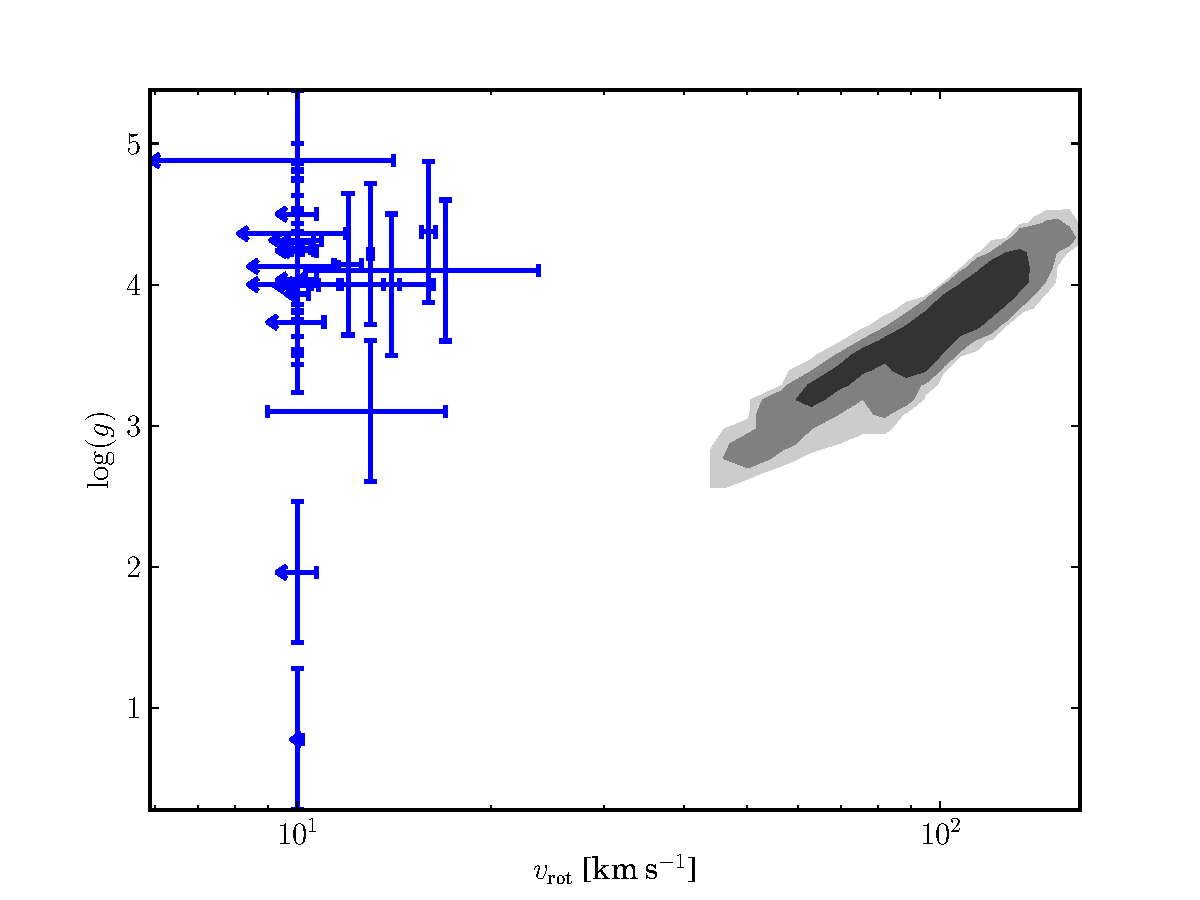
\includegraphics[width=0.7\textwidth]{chapter_sn1006/plots/compare_vrot.pdf} 
   \caption[Comparison of rotation and surface gravity of SN 1006 candidates]{Comparison of the evolutionary state and rotational velocity of 55000 binary synthesis \glsentryname{sds} progenitors \citep[gray shades;data from][]{2008ApJ...677L.109H} with the measured rotation from this work. Due to the resolution of the spectrograph most of these stars only have an upper limit of the rotation speed of $\vrot=10\,\kms$}
   \label{fig:han2008_vrot_compare}
\end{figure}


\begin{figure}[htbp] %  figure placement: here, top, bottom, or page
   \centering
   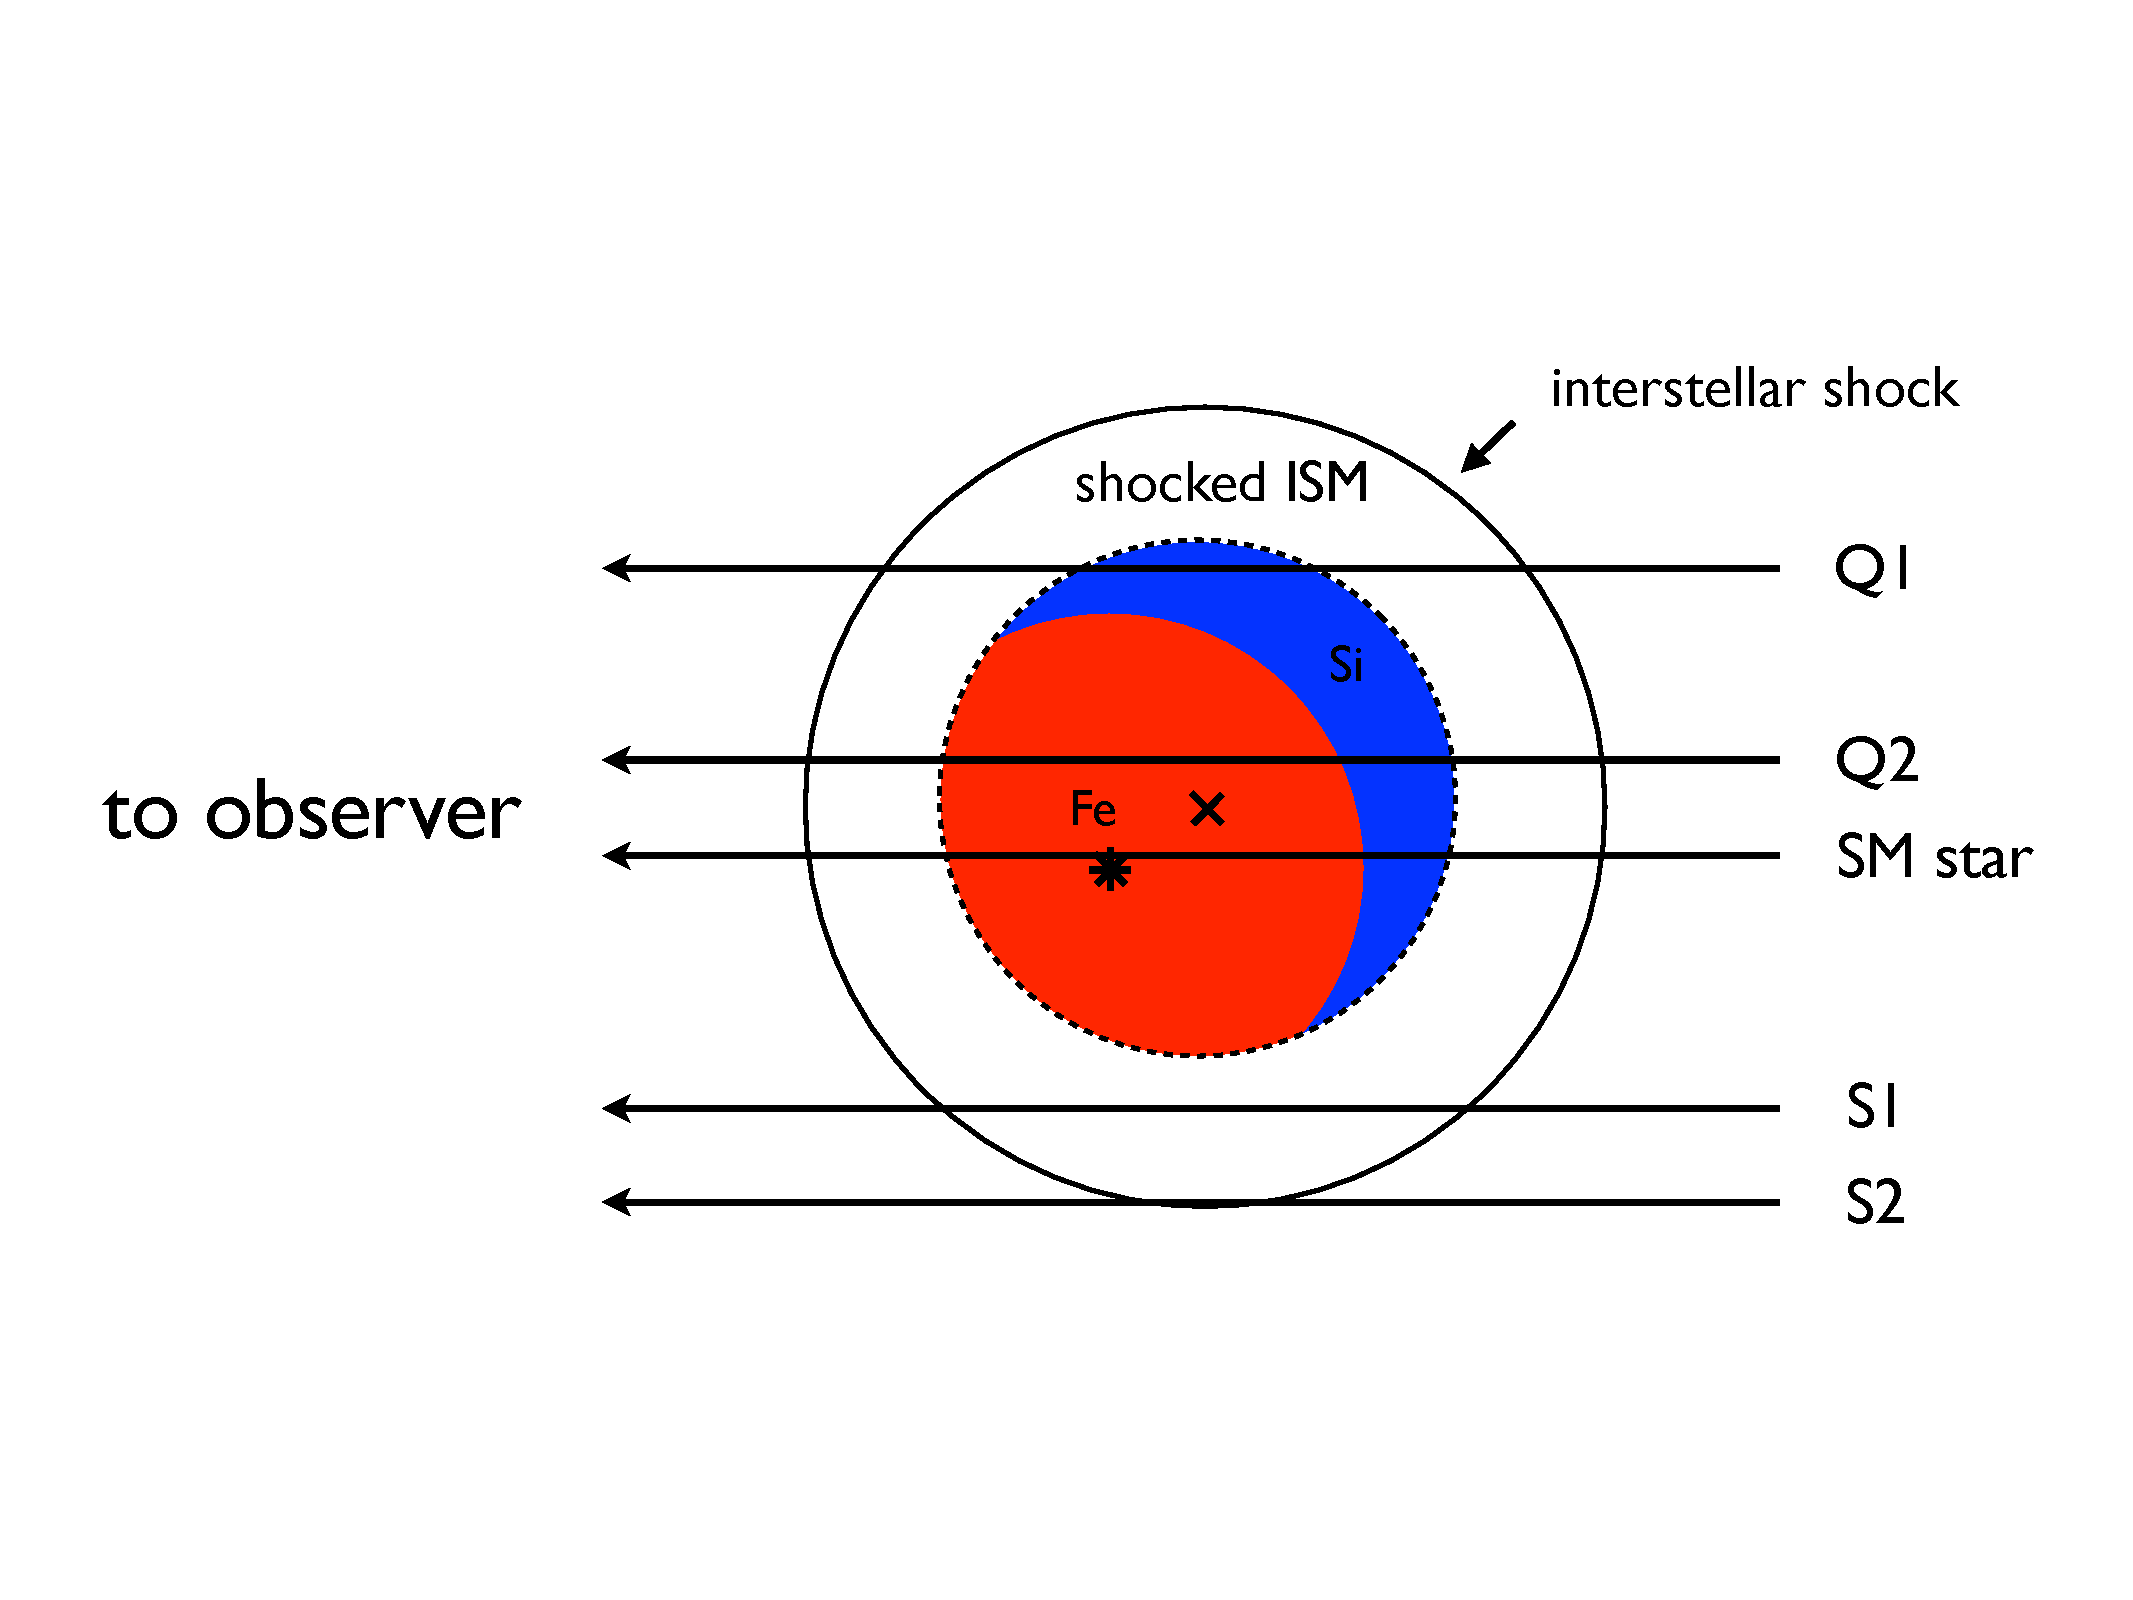
\includegraphics[width=0.7\textwidth]{chapter_sn1006/plots/Winkler2005_probingsn1006_cropped.pdf} 
   \caption[Background UV sources probing the remnant]{Background UV sources probing the remnant. Figure adapted from \citet{2005ApJ...624..189W}}
   \label{fig:sn1006_uvprobe}
\end{figure}

What are the progenitors of \sneia? We have ruled out the standard model of donor stars for \sn{1006}{}. A helium white dwarf as a donor star (see Section \ref{sec:intro_subchandra}) would not be detectable with our method. It is however unlikely that a helium white dwarf would survive the explosion (priv. comm. R\"udiger Pakmor). The other very real possibility is that \sneia\ in general or at least \sn{1006}{} do not have donor stars. A \gls{dds} would definitley explain the observational lack of the thought after companion. 

A last remnant that can be subjected to such an intensive search is Kepler (\sn{1604}). Kepler seems to be different from either \sn{1572}{} and \sn{1006} due to detection of interaction with the \gls{csm}. Observational facts of the Kepler remnant  as well as the description of the donor star search will be discussed in the conclusion of this thesis (Chapter \ref{chap:conclusion}).

